\documentclass{beamer}
\usepackage{pgfpages}
\setbeamertemplate{note page}[plain]
\setbeameroption{show notes on second screen}
% beamer xelatex notes bug workaround, see https://tex.stackexchange.com/questions/232168/normal-text-is-invisible-when-using-beamer-with-notes-and-xelatex 
\makeatletter 
\def\beamer@framenotesbegin{% at beginning of slide
    \usebeamercolor[fg]{normal text}
    \gdef\beamer@noteitems{}% 
    \gdef\beamer@notes{}% 
}
\makeatother
% workaround end **************************************************************
\usepackage[ngerman]{babel}
\usepackage{booktabs}
\usepackage{tabulary}
\usepackage{siunitx}
\usetheme{imise}
\author[Sebastian Stäubert]{Konrad Höffner, Franziska Jahn, Christian Kücherer, Barbara Paech, Birgit Schneider, Martin Schöbel, \textbf{Sebastian Stäubert}, Alfred Winter}
\date[20.9.2017 10:15]{Mittwoch 20. September 2017, 10:15--10:30 Uhr\\
GMDS Jahrestagung, Raum A01 0-006}
\title{Technische Umgebung der SNIK Ontologie\\~}
%\institute{GMDS Jahrestagung 2017}
\subtitle{Ein Semantisches Netz des Informationsmanagements im Krankenhaus}
\newcommand{\todo}[1]{TODO: #1}
\newcommand{\imageslide}[4][]
{
\begin{frame}{#2}
\centering\includegraphics[width=1\textwidth,height=0.8\textheight,keepaspectratio]{#3}
\\#1
\note{#4}
\end{frame}
}

\begin{document}
\begin{frame}
\titlepage
\note{
Publikum motivieren! der Session, Leute sofort begeistern, damit sie nicht einschlafen. 
\begin{itemize}
\item Akzeptanz des Semantic Web in Community der Medizinischer Informatik gestiegen
\item Vielleicht haben Sie ja Daten, bei denen Sie sich nicht sicher sind, ob sich Konvertierung nach Linked Data lohnt und wie aufwändig das ist?
\item Oder sie haben sich bereits entscheiden, wissen aber nicht wie?
\item Technische Umgebung des SNIK-Projekts als Beispiel, viel lässt sich auf andere Anwendungsfälle übertragen 
\item Verwenden von Standardformaten: starke Reduktion von Entwicklungsaufwand durch Verwendung und Adaption existierender Services
\item Gesamte hier vorgestellte technische Umgebung wurde von nur zwei Personen in Teilzeit aufgesetzt. 
\end{itemize}
}
\end{frame}


\imageslide[\url{http://www.snik.eu} \url{http://5stardata.info}]{SNIK Projekt}{img/5star.png}
{
\begin{itemize}
\item kurze Einführung SNIK-Projekt
\item offene Bereitstellung von computerverarbeitbaren Fakten des Informationsmanagements im Krankenhaus aus Lehrbüchern
\item Nutzen maximieren: 5 Sterne Schema für offene Daten von Tim Berners-Lee
\end{itemize}

\begin{enumerate}
\item Rechtssicherheit für Benutzer durch offene Datenlizenz. PDFs der Bücher dürfen allerdings nicht online gestellt werden. Nur wenn jemand fragt:
\begin{itemize}
\item CC BY-NC-SA 4.0 Lizenz (Creative Commons Attribution-NonCommercial-ShareAlike).
\item Erlaubt: Teilen, Adaptieren
\item Bedingungen: Attribution, Nichtkommerziell, gleiche Lizenz für Derivate. Für eine offene Lizenz recht restriktiv, sind aber für andere Optionen offen
\end{itemize}
\item Strukturiertes Format: Lesen der Bücher und manuelles modellieren der Fakten in Tabellen, sehr zeitaufwändig 
\item Stufe 3 trivial: speichern in offenem Format, in unserem Fall CSV
\item Konvertierung der Tabelle zu einer Ontologie mittels Tarql scripts, viel Vorarbeit in Tabellen 
\item Interlinks zwischen Büchern automatisch erstellt durch LIMES
\end{enumerate}
}

\begin{frame}{Einsatz}
\centering
\begin{tabular}{ll}
\toprule
\textbf{Ziel}	&\textbf{Zielgruppe}\\
\midrule
Lehre			&Lehrer und Studenten\\ 
Datenintegration	&Krankenhausleitung, CIO\\
Formalisierung		&Domänenexperten, Ontologen\\
\bottomrule
\end{tabular}
\note{
\begin{itemize}
\item benötigte Tools hängen von Zielen und Zielgruppen ab 
\item Lehre: Vermittlung des Fachwissens an Studenten. Für Vorteil gegenüber/zusätzlich zu Lesen der Bücher: kein Vorwissen, schnelle, simple und intuitive Wissensvermittlung.
\item Datenintegration: Ontologie kann als Vokabular von verschiedenen Anwendungen benutzt werden
\item Verbesserung des durch Studenten extrahierten formalisierten Fachwissens durch Ontologen und Domänenexperten
\end{itemize}
}
\end{frame}

\imageslide[\url{https://github.com/IMISE/snik-ontology}]{Ausgangspunkt: RDF Dump}{img/rdfdump.png}{
\begin{itemize}
\item Nach Erklimmen der 5 Stufen erhalten wir eine RDF/OWL Ontologie, im Bild im RDF/XML-Serialisierungsformat
\item in Metaontologie und Unterontologien aufgeteilt, eine pro Buch/andere Quelle
\item große Ontologie, weist viele Eigenschaften einer Wissensdatenbank mit Instanzdaten auf
\end{itemize}
}

\imageslide[\url{https://protegewiki.stanford.edu/}]{RDF Dump in Protégé}{img/protege.png}{
\begin{itemize}
\item mit RDF Dump kann man nicht viel machen, Ontologen können es z.B. in Protégé bearbeiten (siehe Bild) 
\item viele Ontologieentwickler hören an dieser Stelle schon auf, aber für unsere Ziele nicht genug, da nur für Experten geeignet
\item um Ziele zu erfüllen, haben wir Services entwickelt 
\end{itemize}
}

\imageslide[\url{http://www.snik.eu/sparql}]{SPARQL Endpoint}{img/sparqlresult.png}{
\begin{itemize}
\item Kernservice, auf dem fast alle anderen aufbauen 
\item SPARQL ist defacto-Standard-Abfragespache für Linked Data
\item Experten können selbst abfragen stellen, andere greifen auf Services zu
\item analog zu relationaler Datenbank
\end{itemize}
}


\imageslide[\url{http://www.snik.eu/ontology}]{RDF Browser---LodView}{img/browse-cio.png}{
\begin{itemize}
\item jeder Begriff unserer Ontologie hat eine URL 
\item aufgelöst zu LodView, Detailansicht der Eigenschaften des Begriffs
\item für alle Zielgruppen 
\item RDF besteht aus Tripeln: Subjekt (aufgerufene URL), Prädikat (Spalte links), Objekt (Spalte rechts)
\end{itemize}
}

\imageslide[\url{http://www.snik.eu/graph}]{Graphvisualisierung I}{img/graph-entitytype}{
\begin{itemize}
\item LodView bietet Detailansicht aber keinen Überblick  
\item Eigenentwicklung einer Webapp zur Visualisierung der Ontologie als Graph auf Basis der Cytoscape.js-Bibliothek
\item jeder Begriff ein Knoten (Kreis) im Graph, Beziehungen sind Kanten
\item Farben für unterschiedliche Unterontologien, rot Metamodell 
\end{itemize}
}

\imageslide[\url{http://www.snik.eu/graph}]{Graphvisualisierung II}{img/graph-erf.png}{
\begin{itemize}
\item die üblichen Graphoperationen: kürzester Weg, direkte Nachbarn
\item Suche 
\item Navigation
\item Integration mit anderen Services: RDF Browser für bestimmten Begriff öffnen, Fehler melden, editieren
\item Probieren Sie es selbst! www.snik.eu/graph
\end{itemize}
}

\imageslide[\url{http://www.snik.eu/graph}]{Graphvisualisierung---Spiderworm}{img/spiderworm.png}{
\begin{itemize}
\item Spiderworm: kürzester Weg + alle direkten Nachbarn vom Zielknoten
\item Einsatz in der Lehre
\end{itemize}
}

\begin{frame}{LodLive \& Relfinder}
\centering
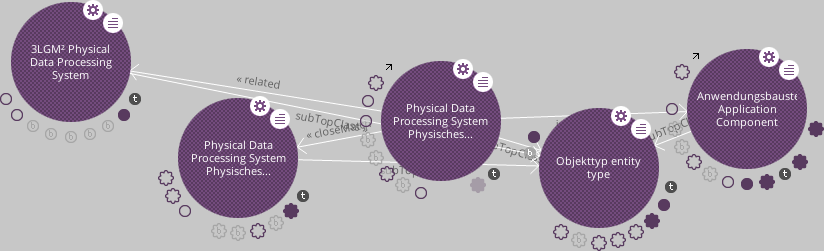
\includegraphics[width=\textwidth]{img/lodlive.png}\\
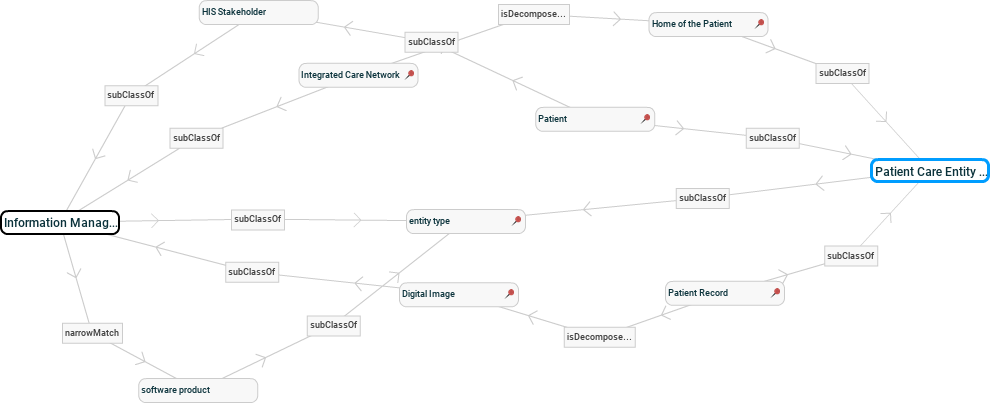
\includegraphics[width=\textwidth]{img/relfinder.png}
\note{
\begin{itemize}
\item über SPARQL Endpunkt kann man auch externe Services anbinden 
\item keinerlei Entwicklungsaufwand für uns
\item Beispiel: LodLive zum schrittweise Graph-Explorieren
\item Beispiel: Relfinder für alle kurzen Wege zwischen zwei Knoten, genaue Beziehung zwischen ihnen
\end{itemize}
}
\end{frame}



\imageslide[https://imise.github.io/snik-ontology/2017/04/12/dashboard]{Statistiken}{img/dashboard-medley.png}{
\begin{itemize}
\item für Fehlersuche  
\item 
\item 
\end{itemize}
}

\imageslide[\url{https://github.com/IMISE/snik-ontology/issues}]{Ticketsystem}{img/gitissue.png}{
\begin{itemize}
\item 
\item 
\item 
\end{itemize}
}

\imageslide[\url{http://www.snik.eu/evaluation}]{TripleCheckMate}{img/triplecheckmate.png}

\imageslide[http://aksw.org/Projects/LIMES]{LIMES}{img/limes.png}{
\begin{itemize}
\item 
\item 
\item 
\end{itemize}
}


\iffalse
\begin{frame}{Interlinking}
\begin{itemize}
\item Verknüpfungen zwischen Klassen verschiedener Ontologien
\item LIMES Tool von AKSW um Axel Ngonga
\item Finden von Kandidaten durch Stringähnlichkeit, manuelle Verifizierung und Kategorisierung
\end{itemize}
\end{frame}
\fi

\imageslide[https://github.com/IMISE]{Öffentliche Softwarerepositories}{img/github.png}{
\begin{itemize}
\item 
\item 
\item 
\end{itemize}
}


\begin{frame}
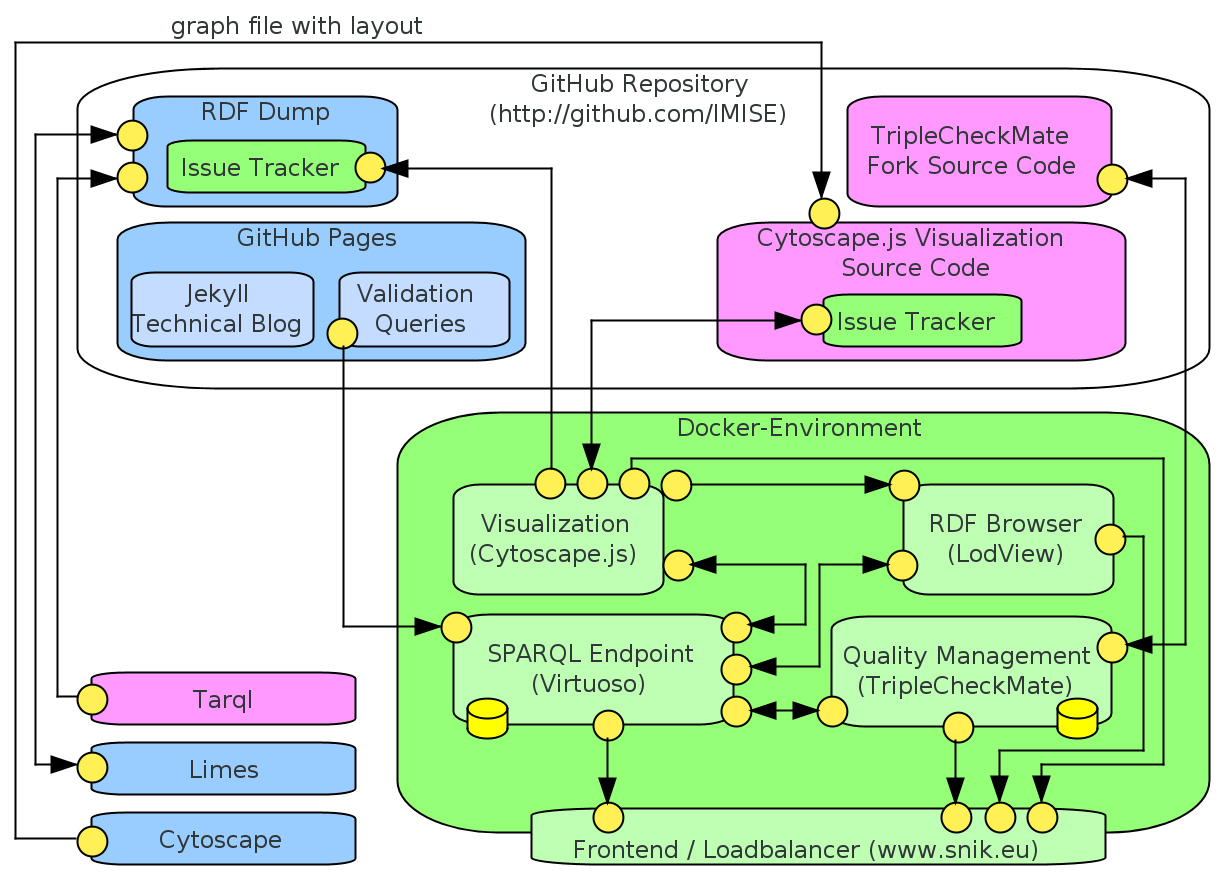
\includegraphics[width=\textwidth]{img/architecture.png}
\note{
\begin{itemize}
\item da kennst du dich ja selbst am besten aus 
\item 
\item 
\end{itemize}
}
\end{frame}

\begin{frame}[fragile]{Fragen?}
\begin{itemize}
%\item Diese Präsentation \url{https://github.com/KonradHoeffner/latex/releases/download/colloquium/colloquium.pdf}
\vspace{0.5em}%here it works as intended
\item Überblick \url{http://www.snik.eu}
\item Visualisierung \url{http://www.snik.eu/graph}
\item SPARQL Endpunkt \url{http://www.snik.eu/sparql}
\item RDF Browser \url{http://www.snik.eu/ontology}
\item Evaluation \url{http://www.snik.eu/evaluation}
\item Twitter \url{https://twitter.com/snik\_proj}
\item Technisches Blog \url{https://imise.github.io/snik-ontology}
\item GitHub Organisation mit Ticketsystem \url{https://github.com/imise}
\end{itemize}
\end{frame}

\end{document}
